% 
% \documentclass[paper=a4,fontsize=12pt,open=right,noabbrev]{report}
% \documentclass[12pt]{report}
% \usepackage[utf8]{inputenc}
% \usepackage{amsmath}
% \usepackage{amssymb}
% \usepackage{graphicx}
% \usepackage{placeins}
% \usepackage{cite}
% \usepackage{physics}
% \usepackage{mathrsfs}
% \usepackage{geometry}
% 
%  \setlength{\parindent}{0em}
% \setlength{\parskip}{1em}
%  
% 
% \begin{document}

 
\chapter{Reweighting Dynamics by Collective Variables} 
Complex systems consist of many particles giving rise to pair and higher order  interactions. The large number of interactions is burdensome to analyse and display for interpretation. One typically reduces the high-dimensional space to a few low-dimensional variables describing the slowest dynamical processes of the system. This reduction implies that the remaining coordinates average out on faster timescales or have no effect on the process of interest. The system is reduced to the chosen aspects and is not under full investigation. Examples are the description of a magnet by its magnetisation whilst ignoring the influence of local dipole fluctuations~\cite{tobik2017free} or the crystallisation of particles described by the closest radial environment of each crystallising particle~\cite{radhakrishnan2003nucleation}.  Fast and local processes are  integrated out when deciding on a set of collective variables. This is compatible with Markov State Model (MSM)  construction because here, fast processes are neglected too. However, the mesoscopic descriptors or \textit{collective variables}(CV) are chosen system-specific and the choice limits the view on the system: The crystallisation described by the local environment of the particles holds detailed view on the crystalline phase but limited information on the liquid phase~\cite{radhakrishnan2003nucleation}. Furthermore, a poor choice of CVs can hide important processes and free energy barriers or cause an inaccurate estimation of implied timescales~\cite{bolhuis2000reaction,valsson2016enhancing,noe2017collective}. Dimensionality reduction and choice of an advantageous set of collective variables is a widely discussed research field on its own and is applied to describe complex systems in chemistry, biology, physics and more~\cite{rohrdanz2013discovering}. 

MSM requires the use of CVs to be computationally accessible. State of the art use $10^2 - 10^3$ microstates~\cite{noe2019markov}, resulting in $10^4 - 10^6$ possible transitions that have to be sampled. A construction on the full conformational space requires a larger number of transitions that would  exceed computational boundaries and we use collective variables to bypass these limitation. This chapter tests the reweighting procedure on systems described by collective variables to extend its scope to a larger group of systems.
The reweighting method is first applied to a particle in a 2D-potential described by a 1-dimensional collective variable. The second test system is a coarse-grained tetraalanine peptide being described by CV and showing many-body interactions.

The reweighting procedure can be applied without adjustment. The collective variables hide the full local entropy productions, but the relative local entropy productions
\begin{equation}
 \Delta S_{ij} - \Delta S_{ij}^q = \frac{ \Delta U(x_j) - \Delta U(x_i) + (x_j - x_i) \Delta f }{k_{\mathrm{B}} T}
 \end{equation}
 is sufficient for reweighting. Here, $\Delta U(x)$ is the change in potential and $\Delta f$ is the change in force of reference and target system. The new potentials or forces are defined for the CVs coordinate $x$, unlike in the previous chapter for the conformational coordinates.  We only need to know the change in local entropy productions $\Delta S_{ij} - \Delta S_{ij}^q$ due to driving from theoretical prediction. Since the forces and potentials are aligned with the CVs we can calculate them. The total local entropy productions $\Delta S_{ij}$ are not known from theory anymore. The total values are sampled by the reference simulation itself. 

\section{Single Particle in Collective Variable Space} 
As a first testing ground we choose the 2D system from section~\ref{sec:2Dsys} and integrate out the $y-$dimension orthogonal to the driving force, shown in figure~\ref{fig:potred}a,b. This will imitate the reduction to a collective variable on the testing ground of the well-understood minimal system. A MSM is constructed on the reduced space.

\begin{figure}
 \centering
 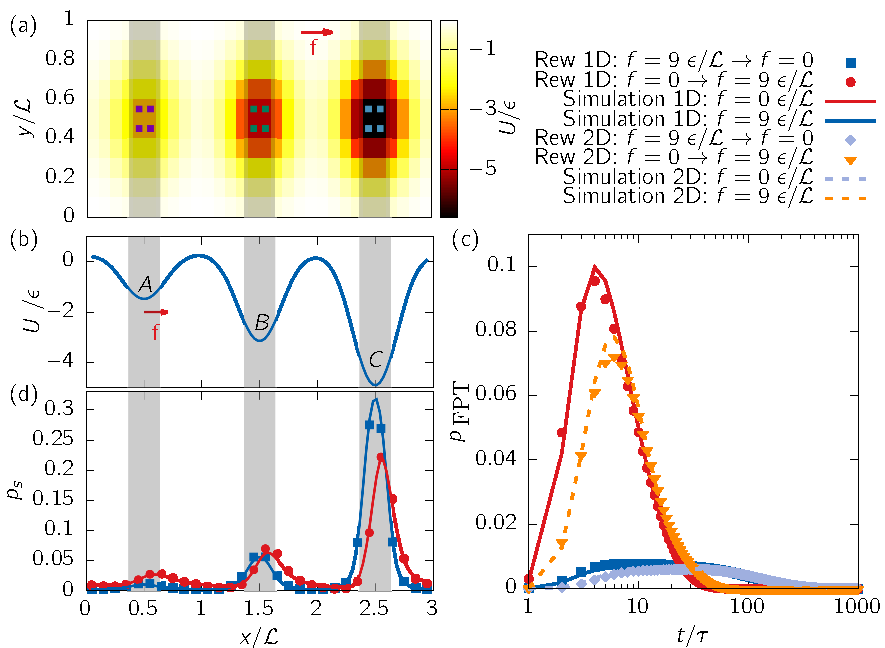
\includegraphics{../plots/Frew/single_1030.pdf}
 \caption[Free energy surface, stationary distribution and first-passage time distribution of a chosen process for the 1D reduced system]{ (a) The 2D potential with the three metastable states indicated by squares. Integrating out the $y-$dimension gives (b) the mean potential of the equilibrium system. The grey area represents the new metastable states $A$,$B$,$C$. The area of the metastable state is effectively increased.  (d) The stationary distribution of the reduced system and (c) FPTD of the process  $C\rightarrow B$. The lines in (c,d) represent the results from simulating a single particle without (blue) and with (red) external force. The dots are the results from reweighting the systems into each other. The orange and light-blue dashed lines show the same process for the underlying 2D process with dots representing the reweighted FPTD.  }
 \label{fig:potred}
\end{figure} 
 
The 2-dimensional system is reduced by integrating along the $y-$axis of the system. A mean force and mean potential is calculated by
\begin{equation}
\begin{aligned}
  \langle \mathbf{F} (x) \rangle &= \int \dd{y} \mathbf{F}_{\text{2D}}(x,y) \pi(x,y) \\
  \langle U (x) \rangle &= \int \dd{y} U_{\text{2D}}(x,y) \pi(x,y) .
\end{aligned}
\end{equation}
Note that the definition of the mean potential is only valid for the equilibrium system and a potential cannot be defined off-equilibrium. The position of the metastable states are determined from the $x$-coordinate of the 2D system to compare the dynamics of full and reduced system. The dimensional reduced data are collected during runtime of the full systems simulation. A MSM is constructed with the same lagtime $\tau=0.02\,\mathcal{T}$ and the same 30 equi-sized microstates in $x$-direction. 

Figure~\ref{fig:potred}c and d compares the first-passage time distribution (FPTD) and the stationary distribution of the reduced system in equilibrium and under driving of $9\,\frac{\epsilon}{\mathcal{L}}$ when reweighting the systems into each other.  The FPTD of the 2D system in full conformational space is shown for comparison. Small deviations are seen in the FPTD, however, they are of the same magnitude and position as the reference 2D system. The reweighting for short processes of $1-5\,\tau$ are overestimated, whereas the peak is underestimated in both cases. The tail for longer processes is reweighted correctly. According to the results shown in figure~\ref{fig:potred}d, the stationary distribution is recreated by the reweighting procedure.  We deduce that the reweighting works well, even though system's details are lost by the used collective variables. An impairing effect on the reweighting cannot be observed for this system.  The mentioned deviations are based on deviations on the reweighting in the underlying 2D-system in full conformational space.
\begin{figure}
\centering
 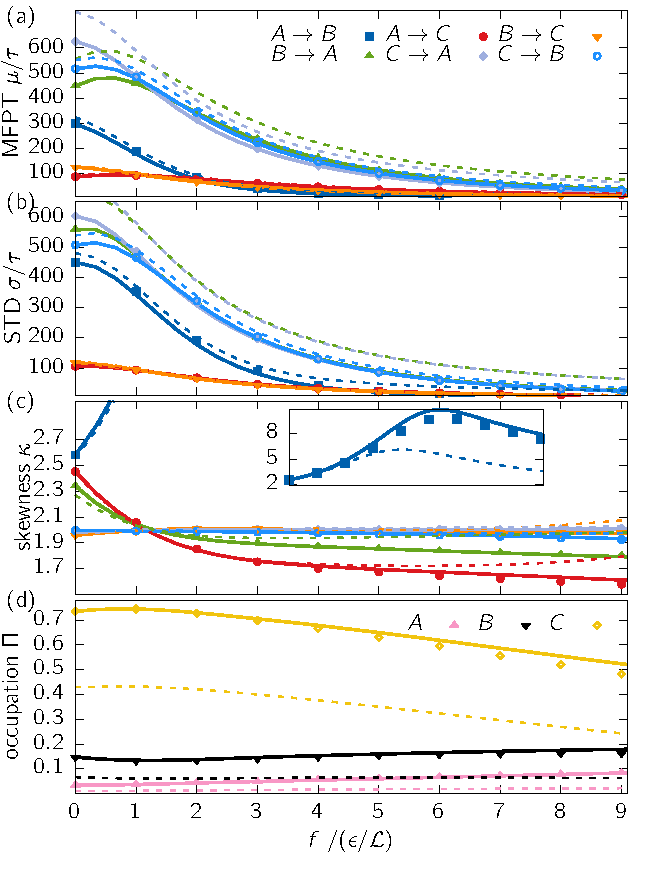
\includegraphics{../plots/Frew/mom_1030.pdf}
 \caption[The first three moments and the population of metastable states for the reduced 1D system for varying driving forces.]{(a-c) The first three moments of the FPTD for all six processes between metastable states defined in figure~\ref{fig:potred}b under varying external force $f$. (d) The occupation probability of each metastable state. The dots represent the value measured from simulation. The line is the equilibrium system continuously reweighted. The dashed lines are the processes of the underlying processes in 2D space.  }
 \label{fig:momred}
\end{figure}

Figure~\ref{fig:momred} shows continuous reweighting from the equilibrium system for the first three moments of the FPTD between metastable states and the occupation probability $\Pi$ of each metastable state. Additionally, the reweighting from the underlying 2D system is shown by dashed lines. First, we focus on comparing results of the 2D system and its reduced system. The mean first-passage time (MFPT) is responding to external driving the same in both systems. The processes along the driving force speeds up immediately. The processes opposing the driving slow down at first, before the spatially longer path along the external force becomes more probable and the process speeds up too. For all processes the 2D process is slower than the coarse-grained process. This effect of accelerated dynamics is known from coarse-graining different materials~\cite{rudzinski2019recent,depa2005speed,guenza2015thermodynamic,meinel2020loss}. It originates in the disappearance of roughness in the free energy surfaces, resulting in a decrease of effective friction and increase of effective mobility. For our simplified model, this effect reduces the effective potential barriers, leading to the acceleration of the coarse-grained process. The response of full and reduced processes under driving remains qualitatively the same although mobility was not preserved.  

The standard deviation (STD) of the FPTD of the reduced system is lower compared to the 2D system. This agrees with the observation that MFPT and STD behave similarly. The skewness of both systems agree. A deviation of the full and reduced system is seen in the inset of the skewness for  process $A \rightarrow B$. The initial increase in skewness was seen for different systems in chapter~\ref{ch:RewU} based on low discretisation of the FPTD for fast processes. The following drop of skewness was unique for the 2D system and is explained by emergence of another peak of slow processes in the FPTD. This class of processes was identified with trajectories bypassing the metastable state due to heavy driving. This effect of bypassing a metastable state cannot occur in the 1-dimensional description.
\begin{figure}[t]
\centering
 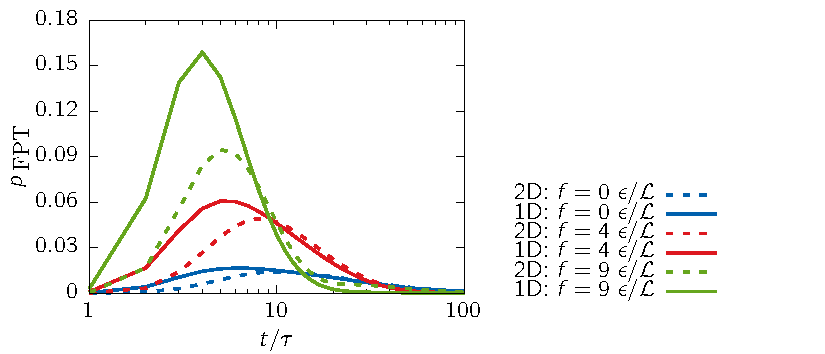
\includegraphics{../plots/Frew/fpt_1030.pdf}
  \caption[First-passage time distribution of transition $A \rightarrow B$ simulated at three different driving forces for the 2D and the reduced model. ]{First-passage time distribution of transition $A \rightarrow B$ simulated at three different driving forces. Increased driving promotes short-time processes and suppresses slow processes. The continuous lines show the FPTD for the reduced system, the dashed lines for the underlying 2D system.   }
 \label{fig:fpt1Dred}
\end{figure}
Figure~\ref{fig:fpt1Dred} shows that the FPTD of the reduced system under driving does not show a second peak. The decrease around $6\,\frac{\epsilon}{\mathcal{L}}$ of the skewness is based on a symmetrising effect on the FPTD of stronger driving. The deviation in skewness of the 2D system and the reduced system is thus based on loss of information of dynamics in $y$-direction  when describing the dynamics by collective variables.  

The occupation probability of the metastable states is considerably larger for the reduced system. The metastable states in the 2D system are smaller because they do not span the whole $y$-direction. The reduction to the $x$-axis enlarges the metastable states effectively and the occupation probability increases. The trend of decreasing occupation in $C$ and increasing occupation $A$ and $B$ is the same for both systems.

In the following, we will discuss to the deviation between simulation of the reduced system and its reweighted properties.  The largest deviation can be seen for the process $A \rightarrow B$, although it is comparable to the deviation of the 2D system for this process shown in figure~\ref{fig:mom2D}. The same observation is made for the deviation in occupation probability of state $C$. The error of the reweighting are much smaller for the other processes. In general the deviations are all of the same shape and relative quantity as for the underlying 2D process. We conclude that the use of collective variables of the system did not affect the reweighting process. Hence, it can be applied to the same extend as the reweighting on configurational space. Deviations of the reweighting are adopted from the underlying errors in configurational reweighting and were discussed in section~\ref{sec:Error}.

From the Maximum Caliber point of view the choice of coordinates does not make a difference. It chooses the system with the most uncertainty, given the prior information and the constraints given --- irrespective of the coordinates. The critical assumptions is made by the CVs: We assume other processes to average out on faster timescales along the process. Here, it means that the fluctuations in $y$-direction average out along the ensemble of trajectories between two basins. It is a reasonable simplification for the present 2D-system, but can be hard to justify for complex systems with other processes involved and more complex CVs. A good choice of CVs is a problem of current research by itself~\cite{rohrdanz2013discovering}. Here, we also have to make sure that the CVs are reasonable for both, the reference and the target system. 




\FloatBarrier

\section{Tetraalanine}
\begin{figure}
\centering
 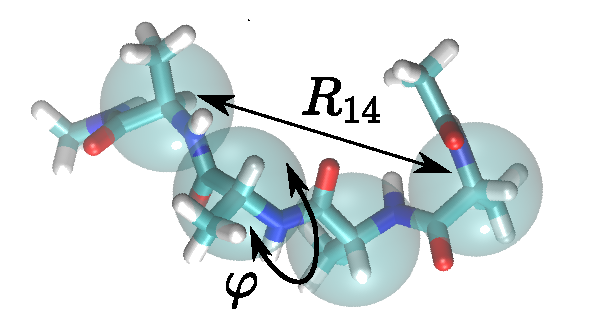
\includegraphics{../images/ala4.pdf}

\caption[Atomistic and coarse-grained representation of the tetraalanine peptide.]{Atomistic and coarse-grained representation of tetraalanine. Atoms are shown as rods,  where turquoise, white, blue, and red represent C, H, N, and O, respectively. The transparent beads show the coarse-grained representation of the system. The end-to-end distance $R_{14}$ and the dihedral angle $\varphi$ are defined for the coarse-grained system. \\
\tiny{Reprinted figure with permission from Tristan Bereau and Joseph F. Rudzinski ,  
Accurate Structure-Based Coarse Graining Leads to Consistent Barrier-Crossing Dynamics, 121(25):256002, 2018 Copyright 2018  by  the American Physical Society. DOI: https://doi.org/10.1103/PhysRevLett.121.256002}}

\label{fig:Ala4}
\end{figure}


\begin{figure}
 \centering
 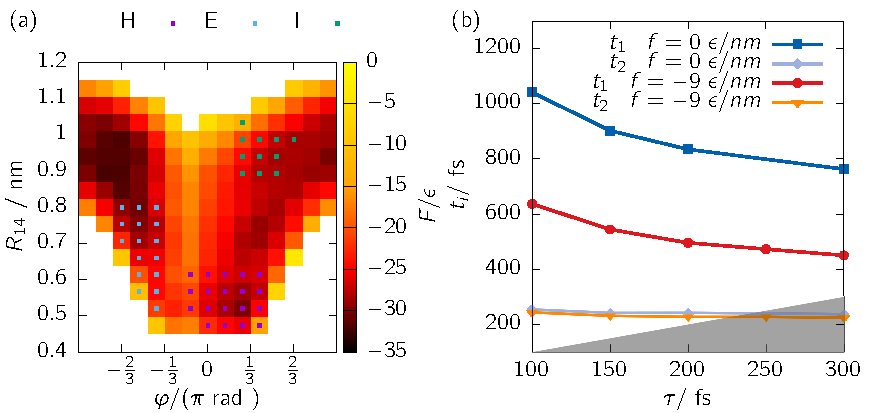
\includegraphics{../plots/Frew/lag_1001.pdf}
 \caption[Free energy surface and lagtime analysis for the two slowest processes of the reference tetraalanine peptide.]{ a) Free energy surface of tetraalanine of the reference system. The metastable states are indicated by H,E,I. (b) Lagtime analysis of the system defined by the reference force field ($f_R=0$) and driven along the end-to-end distance with $f_R = 9\,\frac{\epsilon}{nm}$. The shaded area marks the non-physical area where $t_i < \tau$. }
 \label{fig:AlaLag}
\end{figure}
The following system represents a coarse-grained tetraalanine peptide consisting of four beads.  This model is the first non-artificial material and challenges the reweighting procedure by many-body interactions. External global forces are applied along the CVs to alter the dynamics. These forces may represent an optical tweezer controlling atom distances. The CVs and the forces applied to the system are chosen by the user. The current forces are chosen to test the  effectiveness of the reweighting procedure for conservative and non-conservative forces.

Tetraalanine is a peptide consisting of 44 amino acids and 52 atoms. Each amino acid is coarse-grained to one bead centered at the backbone of the peptide. The coarse-grained force field constructed by Rudzinski and Noid~\cite{rudzinski2015bottom} for the molecule solvated in water consists of 3 pair potentials along the backbone, 2 bending interactions between 3 subsequent beards,  a dihedral angle $\varphi$ between all 4 beads and interaction between the first and the last bead $R_{14}$. The bending interactions are defined by the angle formed between the lines of the first two and last two beads. The dihedral angle is defined by the angle between the planes formed by the first three and last three beads. The MSM is constructed using the end-to-end distance $R_{14}$ and the dihedral angle $\varphi$ as CVs (see figure~\ref{fig:Ala4}), following the example of Bereau and Rudzinski~\cite{bereau2018accurate}. The system will be driven with constant force along both CVs in both directions. The unperturbed system is called the reference system. 
 
The free energy surface of the reference system is shown in figure~\ref{fig:AlaLag}a. Three basins were identified using PCCA+ as introduced in section~\ref{sec:PCCA}. They represent the helical states H, extended state E and one intermediate state I. Note that the direction of driving makes a difference, because the free energy surface lacks the symmetry of the previous systems. The driving along $R_{14}$ can be translated to an additional interaction potential. Systems driven by a force along are still in equilibrium and can be analysed via the eigenvalue decomposition of the transition matrix. Driving along the periodic dihedral angle $\varphi$ will push the system in a non-equilibrium steady state (NESS) that can be analysed using FPTD. 

The lagtime analysis is performed in figure~\ref{fig:AlaLag}b for the reference system and one system driven along $R_{14}$. We choose a lagtime of $200\,$fs to capture the two slowest processes of both systems. The second process is captured by the MSM and is unaffected by the additional forces applied. We expect it to be remain unaffected by larger forces and such it will stay in timescales captured by the MSM. The MSM was constructed with 15 microstates over the range $[-\pi,+\pi]$ in $\varphi$-direction and 15 microstates in the range $[0.45\,\text{nm},1.15\,\text{nm}]$ in $R_{14}$-direction. Two additional sets of microstates were added to collect end-to-end distances outside this range. Energies are given in $\epsilon = \frac{kJ}{mol}$ and the system was simulated at temperature $T = 2.479\,\frac{\epsilon}{k_B}$.

\FloatBarrier
\subsection{Modifying End-to-end Potential}
\label{sec:DrivingEAla}
\begin{figure}
\vspace*{-0.7cm}
\centering
 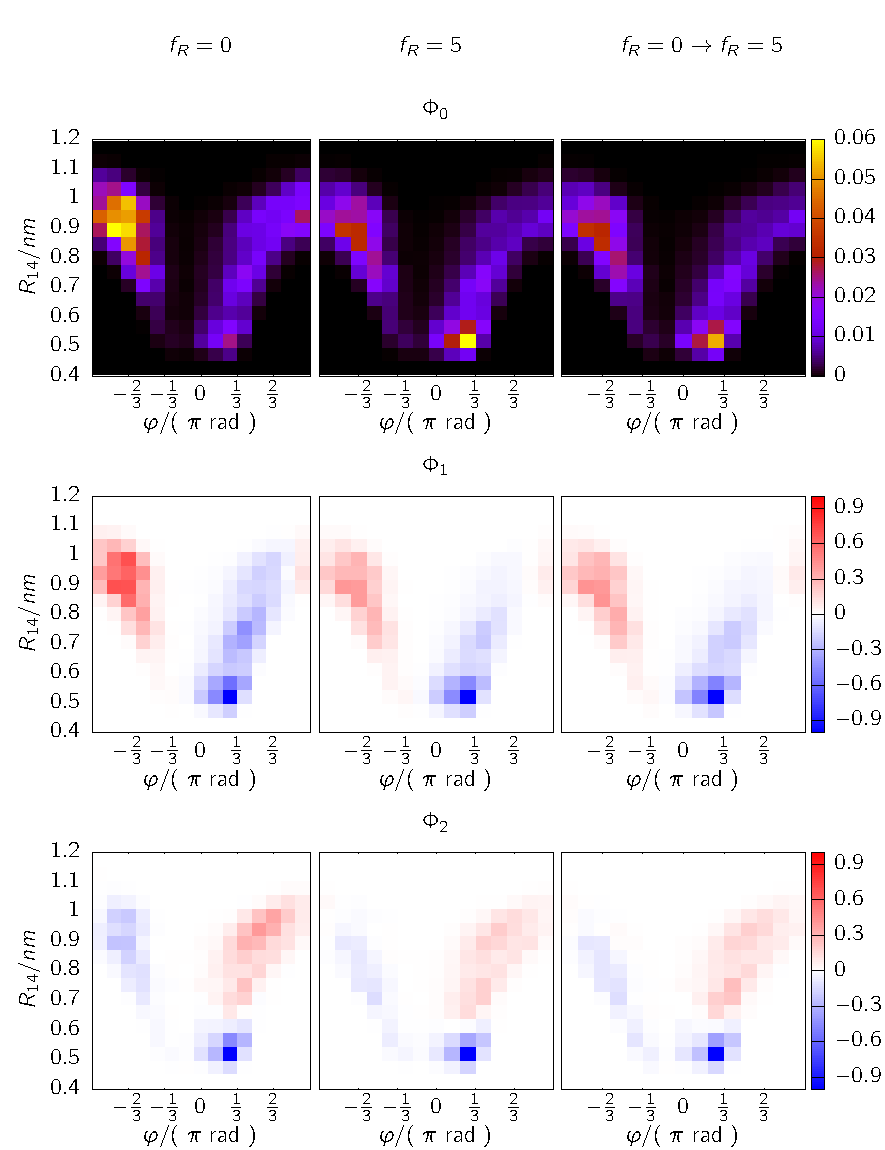
\includegraphics{../plots/Frew/Evec_1002_1902.pdf}
 \caption[Detailed relaxation process analysis of the two slowest processes of the tetraalanine peptide reference model and modified by an end-to-end potential.]{The first row shows the  stationary distribution, the second row the first eigenvector and the third row the second eigenvector of three systems. The system in the first column is the non-perturbed reference system, in the second column the perturbed system at $f=-9\,\frac{\epsilon}{nm}$ and in the third row the reweighted system from reference. }
 \label{fig:EvecAla}
\end{figure}

An optical tweezer uses optical traps to confine beads of a single molecule in harmonic potentials~\cite{jiao2017single}.  We may predict the outcome of such an experiment by applying harmonic potentials of varying strength between the first and the last bead and calculate the effects on statics and dynamics on tetraalanine by reweighting from the undisturbed system. The forces applied are conservative, hence we show an example of reweighting along CVs between equilibrium systems.

At first we have a detailed look at the eigenvectors in figure~\ref{fig:EvecAla} for the system at reference and for driving along $R_{14}$ in negative direction with $f=-9\,\frac{\epsilon}{nm}$. The unperturbed system's stationary distribution shows highest probability at a state with $ \approx 0.9\,$nm end-to-end distance and dihedral angle $\varphi \approx -0.8\,\pi$. This is associated with an extended state. The second minimum can be seen for $\varphi \approx\,0.3 \pi$ and $R_{14} \approx 0.5\,nm$, which is associated with a helical state. A third smaller basin is found at an intermediate state $ \approx 0.9\,$nm and an dihedral angle of $ 0.6\,\pi$. The slowest process describes the transition between the highly populated extended state and the helical and less populated intermediate state over the large barriers around $0\,\pi$ or $1\,\pi$. This second slowest process describes a transition for $\pi>0$ on the right-hand side of the large barrier in the middle, between the helical state and the intermediate state. 


Focusing on the effect of the driving, here, the driving forces the ends together and effectively pushes the stationary distribution to the folded state.  Therefore, the basin of the helical states is more populated than without driving. As shown by the first eigenvector, the slowest process changes and the polymer folds directly in the helical state.  The intermediate state at $0.6\,\pi$ is less important for this process when the additional force is applied. The timescale indicates that the folding occurs faster. The second slowest process is the transition on the right-hand side of the centered barrier and remains unaffected by the driving. We note that 
reweighting to the driven system from the reference system recovers this detailed view on the slowest process correctly.


\begin{figure}
\centering
 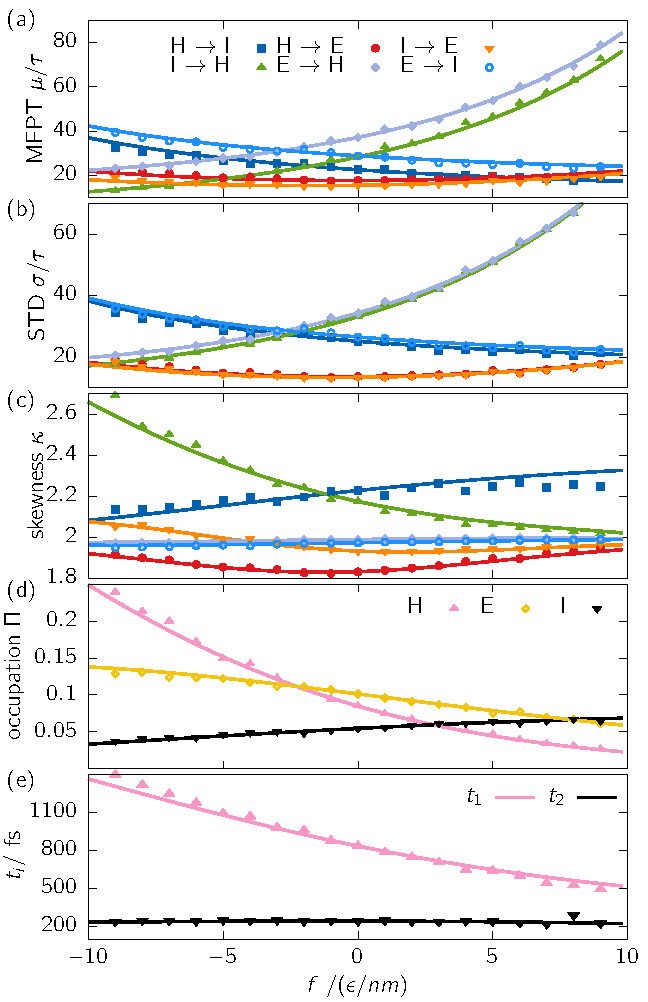
\includegraphics{../plots/Frew/mom_1001.pdf}
 \caption[The first three moments, the population of metastable states and the first two timescales for the tetraalanine peptide for varying driving along the end-to-end distance.]{(a-c) The first three moments of the FPTD for all six processes between metastable states defined in figure~\ref{fig:AlaLag} under varying external force $f$. (d) The occupation probability of each metastable state. (e) The timescale of the two slowest processes covered by the MSM. The dots represent the value measured from simulation. The line is the reference system continuously reweighted.   }
 \label{fig:momAlaR}
\end{figure}


 Figure~\ref{fig:momAlaR} shows the first three moments of the FPTD between the metastable states as defined in figure~\ref{fig:AlaLag}a. The metastable states as defined by PCCA+ do not coincide with the states highlighted for the eigenvectors. State H can be associated with  helical states, located to the right of the free-energy barrier at $\varphi \approx 0.15\,\pi$. State I is an intermediate state at $\varphi \approx 0.4\,\pi$. The global basin at extended state is not covered by the choice of PCCA+ because it is dynamically unstable. Nevertheless, we call the state identified below  extended state E. Transition from H or E to the intermediate state I slow down for attracting end-beads (negative forces) and speed up for repulsive end-beads (positive forces). The inverse happens for the processes from E or I to folded state H. Attractive end-beads increase the speed of these processes, driving to elongated states reduces it. H is the more stable configuration for negative driving because the end-beads can be close together. Transitions to extended state E are comparatively unaffected by the driving. Looking at figure~\ref{fig:momAlaR}d, the stationary distribution shows an increase in population of intermediates state I under repulsive end-beads. The extended state allows the end beads to be far apart and, therefore, it becomes more populated than state H or E.  The intermediate  state I and extended state E change linearly in probability with changing end-to-end attraction, the state H exponentially. The STD behaves proportional to the MFPT. The STD  shows minor changes under driving but does not show peculiar effects as seen for previous systems. The comparison is extended by the first two timescales of the system. The fast timescale depends strongly on the driving, the second timescale is unaffected as we have previously observed in the lagtime analysis. The systems analysed are in equilibrium and the dynamics are governed by accustomed detailed balance, so effects based on path-dependence are not expected. 
 
 The reweighting method works well for the tetraalanine system driven by a constant conservative force. Deviations are increasing for larger forces. This is based on high populations of regions with large and small end-to-end-distance, that are poorly sampled in the reference system. It is concluded that dynamics can be reweighted along the CV even if complex interactions of many bodies are involved.  This is based on the CVs chosen for the system give a reasonable representation for the dynamics of the system. The Maximum Caliber chooses the most uncertain system based on the information it gets. If the CVs chosen to describe the dynamics were insufficient, the Maximum Caliber would rely on insufficient data and produce wrong results. On the other hand, using information on the full conformational space would certainly include  irrelevant information for the chosen constraints. The Caliber would select highest uncertainty for these information. If the constraints were chosen correctly, this does not influence the result on the processes we are interested in. Well-chosen CVs delete information that the Caliber would ignore anyway, but we do not have to sample such information in the first place. In fact, the Maximum Caliber can be applied to choose CVs~\cite{smith2018multi,tiwary2016spectral}. The second input for the Caliber, the change in local entropy productions, can be estimate correctly because the driving is along a CV. Model-specific details on the trajectories --- like the density of trajectories or their local fluctuations --- are contained in the reference data. The new forces in CV space have to be applied to each of them irrespective of such details. 

\FloatBarrier
\subsection{Driving along Dihedral Angle}
\label{sec:DrivingDAla}
\begin{figure}[h]
 \centering
 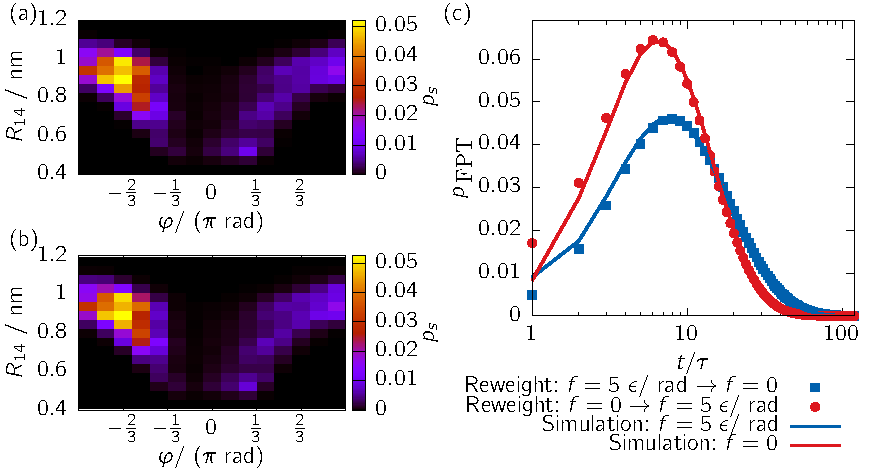
\includegraphics{../plots/Frew/single_2001.pdf}
 \caption[Stationary distribution and first-passage time distribution of a chosen process for tetraalanine peptide driven along the dihedral angle.]{(a) Simulated stationary distribution at $f = 0.8\,\frac{\epsilon}{\footnotesize{\text{rad}}}$. (b) Reweighted stationary distribution from reference to $f = 0.8\,\frac{\epsilon}{{\footnotesize \text{rad}}}$. (c) FPTD of driven and reference system for transition $H \rightarrow E$. The lines show data from simulation, the dots are from reweighting the systems into each other.}
 \label{fig:single2001}
\end{figure}



We will now turn to a driving along the dihedral angle. This is a circular motion with periodic boundary conditions giving rise to a NESS. While this force is artificial for the tetraalanine, such circular forces appear in molecular rotary motors. The rotation is driven by ATP-synthesis giving rise to a unidirectional motion of the molecule~\cite{fillingame1999molecular}.

The system is driven along the dihedral angle in both directions. Figure~\ref{fig:single2001} gives a detailed look at the system driven with $f =\,0.8 \frac{\epsilon}{{\footnotesize\text{rad}}}$. We note that the unfolded states are more populated than before and states to the right of the barrier are less populated. The FPTD distribution from helical states H to the extended state E is shown and captured by the reweighting procedure. Deviations can be seen for short processes of length  $1\tau$.  

\begin{figure}
\centering 
 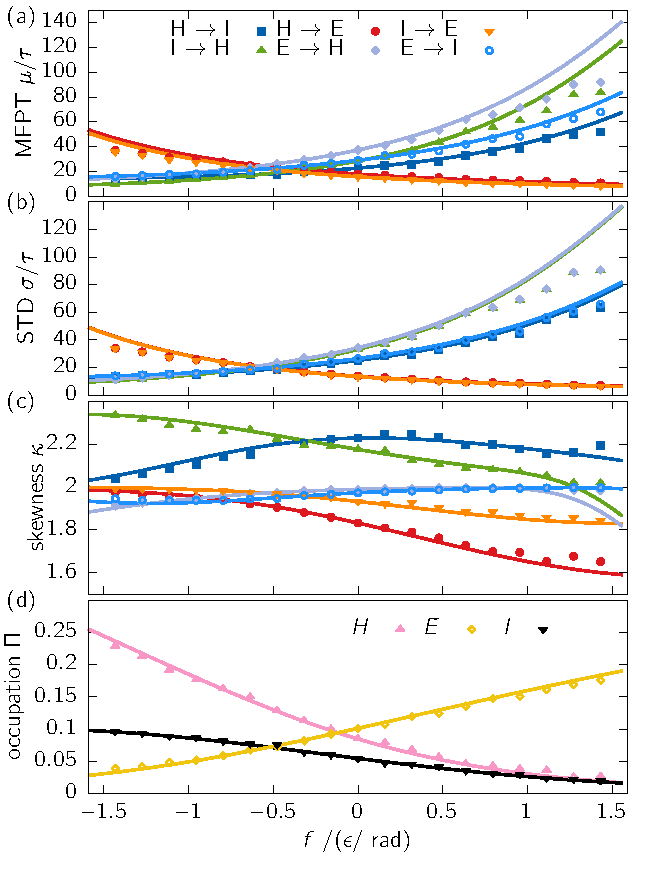
\includegraphics{../plots/Frew/mom_2001.pdf}
 \caption[The first three moments and the population of metastable states for the tetraalanine peptide for varying driving along the dihedral angle.]{(a-c) The first three moments of the FPTD for all six processes between metastable states in figure~\ref{fig:AlaLag} under varying external force $f$. (d) The occupation probability of each metastable state. The dots represent the value measured from simulation. The line is the reference system continuously reweighted.   }
 \label{fig:mom2001}
\end{figure}

Turning to figure~\ref{fig:mom2001} shows the driving along $\varphi$ in both directions. The dynamics of the system are largely dominated by its large centered free-energy barrier. Driving in positive direction, the processes H $\rightarrow$ E and I$\rightarrow$E become faster as they are connected along the periodic boundary.  The process I$\rightarrow$H slows down as it runs opposite to the force. On the other hand H $\rightarrow$I slows down, despite the fact that it runs along the external force. The trajectories bypass the state I under driving more frequently. The transitions I $\rightarrow$H and E $\rightarrow$H are not correctly recovered for larger driving by the reweighting. As expected, the dynamics slow down for simulation and reweighting for low forces. The simulation shows that the curve eventually reaches a maximum since the large barrier is crossed more frequently.  The reweighting procedure has problems capturing this effect correctly although it worked well for the single particle models. The STD follows the behaviour of the mean again and the skewness indicates that the reweighting works well for $|f|  <1\,\frac{\epsilon}{{\footnotesize\text{rad}}}$. Driving in negative direction the effect on dynamics is inverted. Processes aligned with the force speed up, whereas opposing processes are slowing down. The process H$\rightarrow$I does not follow this trend because it is accelerating too. The trajectories normally bypassing the state are now pushed into occupying the state. This is indicated by the increasing population of intermediate state I under negative driving  and depopulation under driving positive driving. The helical state population shows the same behaviour; the extended state shows inverse behaviour. The populations are recovered well by the reweighting, despite the deviations in the dynamics.  


\begin{figure}[t]
 \centering 
 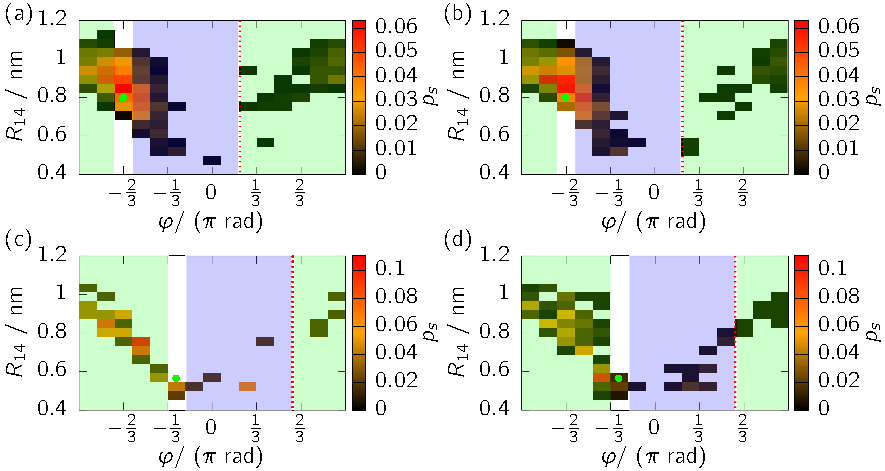
\includegraphics{../plots/Frew/Tv.pdf}
 \caption[Transition matrices of chosen initial point for the tetraalanine peptide reference model and a model driven along the dihedral angle. ]{Transition matrices, starting at the state marked by the green dot. The transition matrices left (a,c) show the reference systems, the right (b,d) show a system driven by $1.4\,\frac{\epsilon}{{\footnotesize\text{rad}}}$. The red line represents the discontinuity in local entropy productions, starting from the marked initial state. All states shaded green are connected to the starting state by trajectory going left, all states shaded blue are connected by a trajectory going right.  }
 \label{fig:dS}
\end{figure}
The reason for the described outlier lies in the local entropy productions. The correct choice is determined by the external force and the set of paths connecting every pair of microstates with each other. This connection of two microstates was straightforward to find for the previous system because they were separated by three or more barriers, as discussed in section \ref{sec:1Dmodel}. It was simple to determine if the collection of paths were directed with or against external forces. Such path dependence cannot occur for driving in $R_{14}$-direction in the previous section, because the origin of a path can be determined without periodic boundaries. This model on the other hand is driven to a NESS with periodic boundaries and shows only one major barrier along the dihedral angle. Choosing the correct local entropy production is more challenging here. For every jump in the Markov Model we have to decide if the underlying trajectory is aligned or directed against the external force. One approach to determine this is to analyse the trajectories as will be shown in section~\ref{sec:Trajectory}. Often one can deduce these information from the transition matrix as demonstrated in figure~\ref{fig:dS}a for the reference system. All states to the right (blue shaded) of the starting point are expected to emerge from trajectories in positive $\varphi$-direction, all states to the left (green shaded) in negative $\varphi$-direction,  taking periodic boundaries into account. In between these sets of trajectories is an area where no transition occurs. The lagtime of the MSM was chosen to be small such that these transitions do no take place, otherwise we were not able to tell whether the transitions occurred via a path going to the left or the right. This empty space acts as a dividing line between the two sets of trajectories, marked by the red dashed line. The connection between the states in the transition matrix indicate where to define the discontinuity in local entropy productions. Figure~\ref{fig:dS}b shows  the transition matrix with driving of $f = 1.4\,\frac{\epsilon}{{\footnotesize\text{rad}}}$ from the same  starting point as before. The transition probabilities change by the driving but the spatially long transition are still forbidden. We are able to tell if the transition took a path in negative or in positive $\phi$-direction. This is essential for the reweighting algorithm to work. For easier understanding it helps to have a look at the starting point of the transition matrix left to the large central barrier in $\varphi$-direction for the same systems in figure~\ref{fig:dS}c,d. The space can be separated in transition in positive and negative $\phi$-direction for the reference system, marked by the blue and green area. For the driven system however, we cannot decide if the Markovian jumps occur from hopping over the barrier or following a path around the periodic boundary. It might be that the microstates are connected by both sets of path. This makes it impossible to calculate the change in local entropy productions. Only if the set of paths are well-separated this is easily possible, as demonstrated for the first starting point. This is the source of the deviation seen in figure~\ref{fig:mom2001} for heavy driving.

We deduce that the reweighting along the dihedral angle will be limited for the present system. The set of paths connecting two microstates should consist of similar trajectories for reference and target systems.  The current system consisting of a single large barrier makes this difficult. Unfortunately, one cannot predict whether the aforementioned conditions are met. The small gaps between the groups of trajectories in Figure~\ref{fig:dS}a,b are a warning signal. Models with three or more barriers, as constructed as a toy model, are less susceptible for this problem. A particle crossing a barrier is expected to take the short path over one barrier and is unlikely to hop over two barrier within one lagtime. We may suspect that this problem occurs more frequently in small model systems with only few particles and less complex free energy surfaces. 

A possible way of solving this problem is by shortening the lagtime of the MSM. Shorter lagtimes result in shorter trajectories and shorter jumps. The reweighting procedure could be applied in a wider range. Unfortunately, figure~\ref{fig:AlaLag} shows that smaller lagtimes show non-Markovian dynamics. At the same time, increasing the number of microstates does not allow us to decrease the lagtime. Other choices made to construct the MSM are the CVs and the microstates. We may select a different second CV when reweighting along the first. Such choices have great impact on the system and solve the problem of missing free energy barriers.  The microstates in the present model are discretised in equal size along the CVs. Advanced clustering techniques like k-means~\cite{likas2003global} or k-medoids~\cite{park2009simple} help to define more complex sets of microstates that would allow to reduce the lagtime. Both, the selected CVs and the way of clustering the CV influence how dynamics are described by the MSM. We noted that the connection of two microstates should be described by a unique bundle of paths. This means that the CVs and its separation in microstates should be chosen to reflect underlying kinetic distances of the system. The same requirement for reweighting of dynamics in equilibrium was noted by Voelz et al.~\cite{wan2016maximum}.

We conclude that the reweighting procedure works for complex many-body-systems described by CVs. We show how the reweighting can be applied for conservative or non-conservative forces along the chosen CVs similarly. These forces might emerge from optical tweezers, molecular motors, mechanical dragging or any other type of disturbance. The reweighting is based on the combination of Maximum Caliber, information on reference data and local entropy productions on the target system. The CVs challenged the procedure by reducing the amount of information to a few variables. We have discussed for the driving along the end-to-end distance in section~\ref{sec:DrivingEAla} that the Maximum Caliber works irrespective of the coordinate system, provided the CVs contain the important information on the process of interest. In this section we have seen how the result is flawed based on inadequate constraints, whereas the underlying data is sufficient. Here, the physical choice of constraints is expected to be correct, but the constraints are flawed from a MSM construction point of view. 

% \FloatBarrier
% \bibliography{/home/marius/PhD/Thesis/references.bib}
% %\bibliography{../references}
% \bibliographystyle{plain} 
%  \end{document}    
